% (C) Marc Lijour, 2019 
% Licensed under a Creative Commons License BY-SA
% https://creativecommons.org/licenses/by-sa/2.5/ca/
% Presentation for the Blockchain Developer Certificate students at George Brown College
% Second part of a lecture on stable coins
% Case study: Basis
% Regulations
% Lessons learned



% ======================================================================================================
%                         Case study: Basis 
% ======================================================================================================
% 

\section{Case study: Basis}

\frame{
    \frametitle{Basis: a price-stable cryptocurrency with an algorithmic central bank}
    Basis (formerly Basecoin) was proposed as a stable coin relying on algorithms.
    The coin could be pegged to any asset or basket of assets.\\
    \vspace{1em}
    The Basis white paper (\citeyear{basis:whitepaper}) is available at \url{https://www.basis.io/basis_whitepaper_en.pdf}
}

\frame{
    \frametitle{The reveal}
    \begin{block}{From Coindesk (\citeyear{coindesk20171013:basecoin})}
    An all-star cast of investors has backed a little-known startup behind a token called basecoin.\\
    \vspace{1em}
    Scheduled to debut with a white paper release on Tuesday, the project, the first from Intangible Labs, boasts investors including 1confirmation, Andreessen Horowitz, Bain Capital Ventures, Digital Currency Group, MetaStable Capital, Pantera Capital and PolyChain Capital.
    \end{block}
}

\frame{
    \frametitle{The vision: an autonomous and decentralized central bank}
    \begin{exampleblock}{From the white paper}
    ``Basecoin would present the world with both the technology and the opportunity to develop an independent, transparent and potentially more stable monetary policy than anything that’s ever been possible via central bank''
    \end{exampleblock}
}

\frame{
    \frametitle{The team}
    \begin{itemize}
        \item Nader Al-Naji, ex Software Engineer at Google, Princeton Computer Science and Maths
        \item Lawrence Diao, ex Software Engineer at Google, Princeton Computer Science Summa Cum Laude
        \item Josh Chen, ex machine learning engineer, Princeton Computer Science Summa Cum Laude
        \item Susan Sidd, ex Managing Director and Legal Director at Goldman Sachs, JD from Harvard
        \item and other \url{https://www.basis.io/\#team}
    \end{itemize}
}

\frame{
    \frametitle{the project}
    In June 2017, there were only a handful of stable coins (Tether, BitShares/BitUSD). Maker DAO would issue its white paper later, in the last month of 2017.\\
    \vspace{1em}
    Today, more than 50 stable coins have been identified (\citeauthor{alyzesam2019:completeguidestablecoins}, \citeyear{alyzesam2019:completeguidestablecoins}).
% https://blog.bitmex.com/a-brief-history-of-stablecoins-part-1/
% https://hackernoon.com/2019-complete-stablecoin-guide-0n9es3zab
}

\frame{
    \frametitle{The technology}
    Basis is not backed by fiat or cryptocurrencies. It relies on \href{https://en.wikipedia.org/wiki/Seigniorage}{Seigniorage} (and \href{https://en.wikipedia.org/wiki/Demurrage\_(currency)}{Demurrage}) principles and algorithms.\\
    \vspace{1em}
    %Basis remains stable by incentivizing traders to buy and sell Basis in response to changes in demand. These incentives are set up through regular, on-chain auctions of “bond” and “share” tokens, which serve to adjust Basis supply.
    The protocol would watch indices (e.g. US Dollar). It would leverage oracles to contract/expand its token supply to control its token value (e.g. exchange rate with the US Dollar).\\
    \vspace{1em}
    Three tokens:
    \begin{itemize}
    \item basecoin is the first token considered, pegged to 1 USD
    \item base bonds used to managed the volatility of basecoin
    \item base shares idem
    \end{itemize}
}

\frame{
    \frametitle{Governance and use of the proceeds}
    They included a return of capital clause in their papers for the raise (see next slide).
}

\frame{
    \frametitle{ICO (fundraising) process}
    Basis raised \$133 million from VCs including Andreessen Horowitz and Bain Capital Ventures.\\
    \vspace{1em}
    The project ended December 13, 2018 with a letter available on the first page of the website at \url{https://www.basis.io}.\\
    \vspace{2em}
    Basis returned the money to investors.
}


% ======================================================================================================
%                         Regulations 
% ======================================================================================================
% 

\section{Lessons learned}
\frame{
    \frametitle{Securities regulation}
    Basis (the coin) wasn't viewed as securities by the US regulator, but the bond and share token were.\\
    Therefore, only accredited investors should be allowed to participate, hence the need for a centralized system to manage access. 
    This impacts not only security but liquidity.\\
    \vspace{1em}
    To make matters worse, this 12-month restriction after the security is issued would be permanent for Basis tokens, since they would be issued on a continuous basis.
}

\frame{
    \frametitle{What went wrong?}
    \begin{center}
    {
    \Huge
    Discussion
    }
    \end{center}
}

% ======================================================================================================
%                         Lessons learned 
% ======================================================================================================
% 

\section{Lessons learned}

\frame{
    \frametitle{Alternative paths}
    Maker DAO uses Collateralized Debt Positions (CDPs). We'll discuss the white paper shortly.\\
    \vspace{1em}
    \href{https://umaproject.org}{UMA} uses facilities to issue non-fungible tokens (contrary to Maker DAO) and actively pursues research on securing oracles with economic incentives.
    % https://twitter.com/hal2001/status/1149466877543845888?lang=en
}

\frame{
    \frametitle{Central Banks are paying attention}
    Christine Lagarde (former head of the IMF and now at the ECB) has been keen to the use of Blockchain by central banks (\citeyear{lagarde2017}).
    The IMF has published a staff discussion note on the topic of Central Bank Digital Currencies (\citeyear{imf2018:cbdc}).\\
    \vspace{1em}
    Potential benefits:
    \begin{itemize}
        \item financial inclusion
        \item security and consumer protection
        \item privacy
    \end{itemize}
    \vspace{1em}
    Obviously, there are also risks for central banks: loss of control on currency, inability to remain the lender of last resort\ldots 
}

\frame{
	\frametitle{The Bank of Canada}
	\begin{figure}
        \centering
		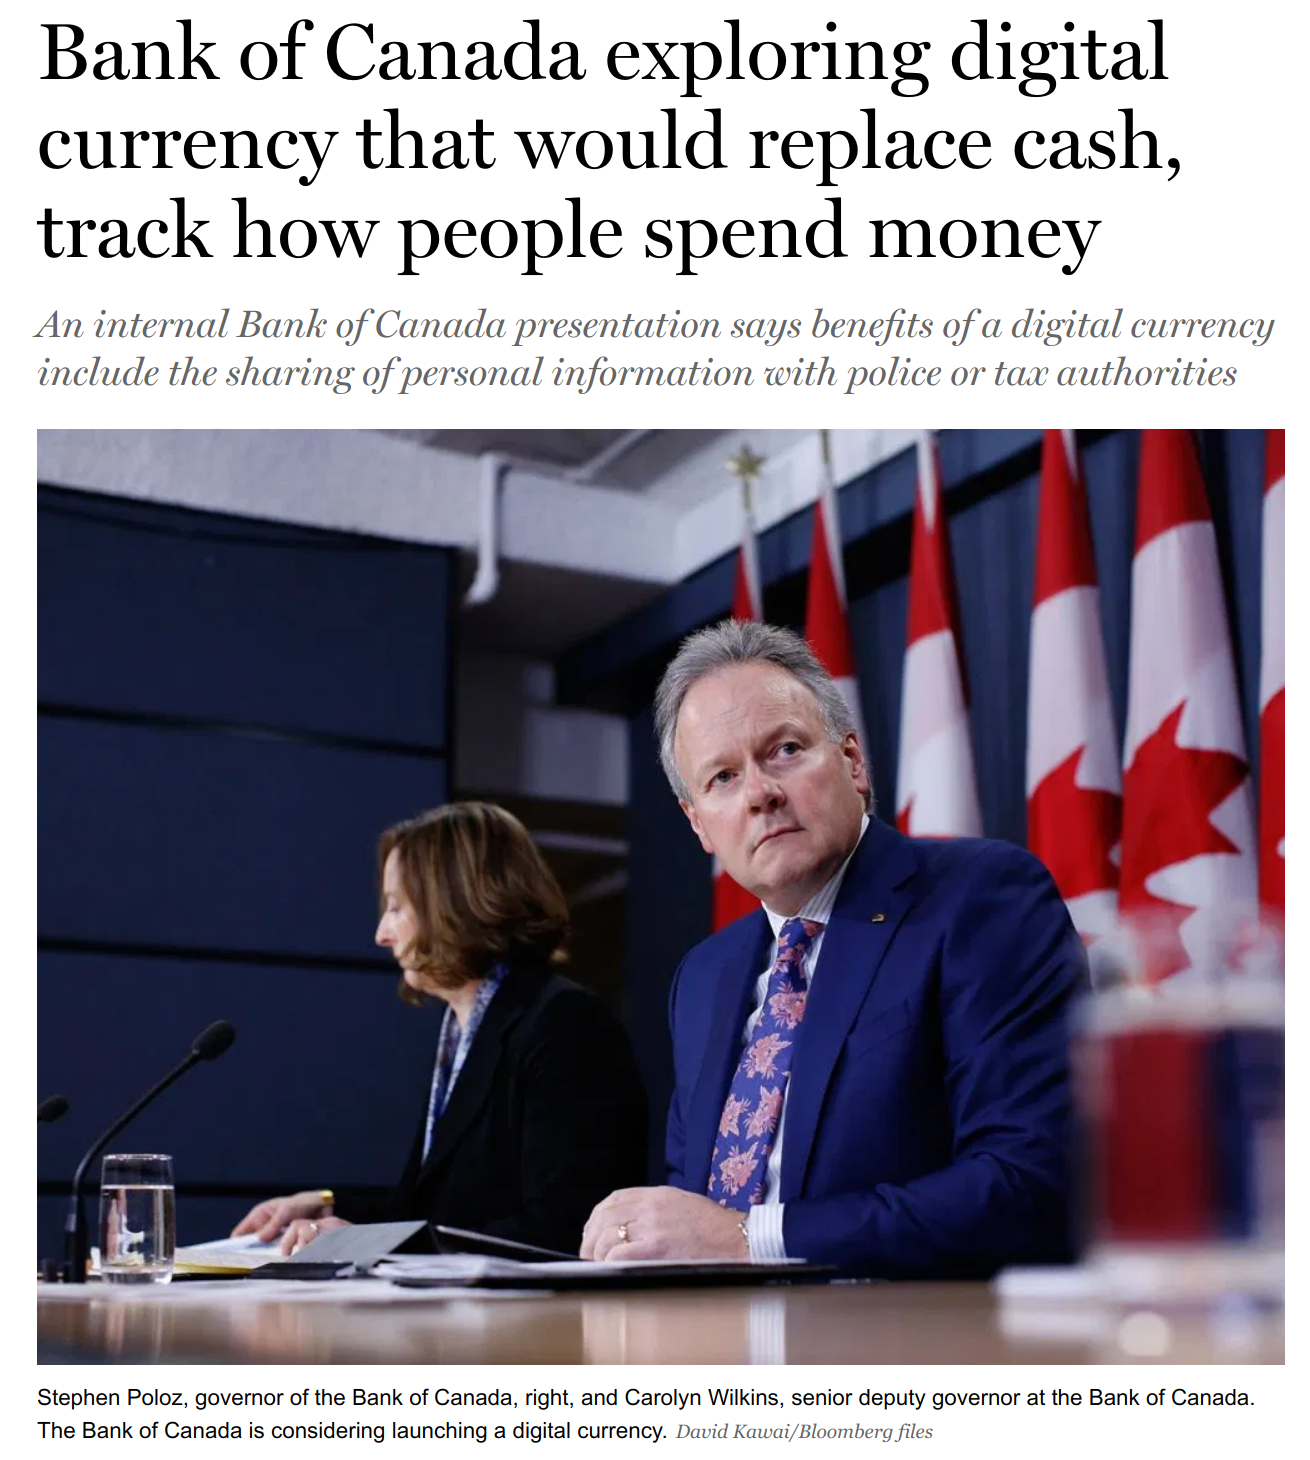
\includegraphics[height=5.5cm]{../pics/cryptocurrency/financialpost-bankofcanada-crypto2019}
        \caption{\cite{financialpost2019:bankofcandacrypto}}
%        \caption{\url{https://business.financialpost.com/technology/blockchain/bank-of-canada-exploring-digital-currency-that-would-replace-cash-track-how-people-spend-money}}
	\end{figure}
    The Bank of Canada has explored the digital currency space since 2012.
    Current discussion involves sharing information with law enforcement and tax authorities.
}

\frame{
  \frametitle{The Bank of Canada (Feb 2020 update}
	\begin{figure}
        \centering
		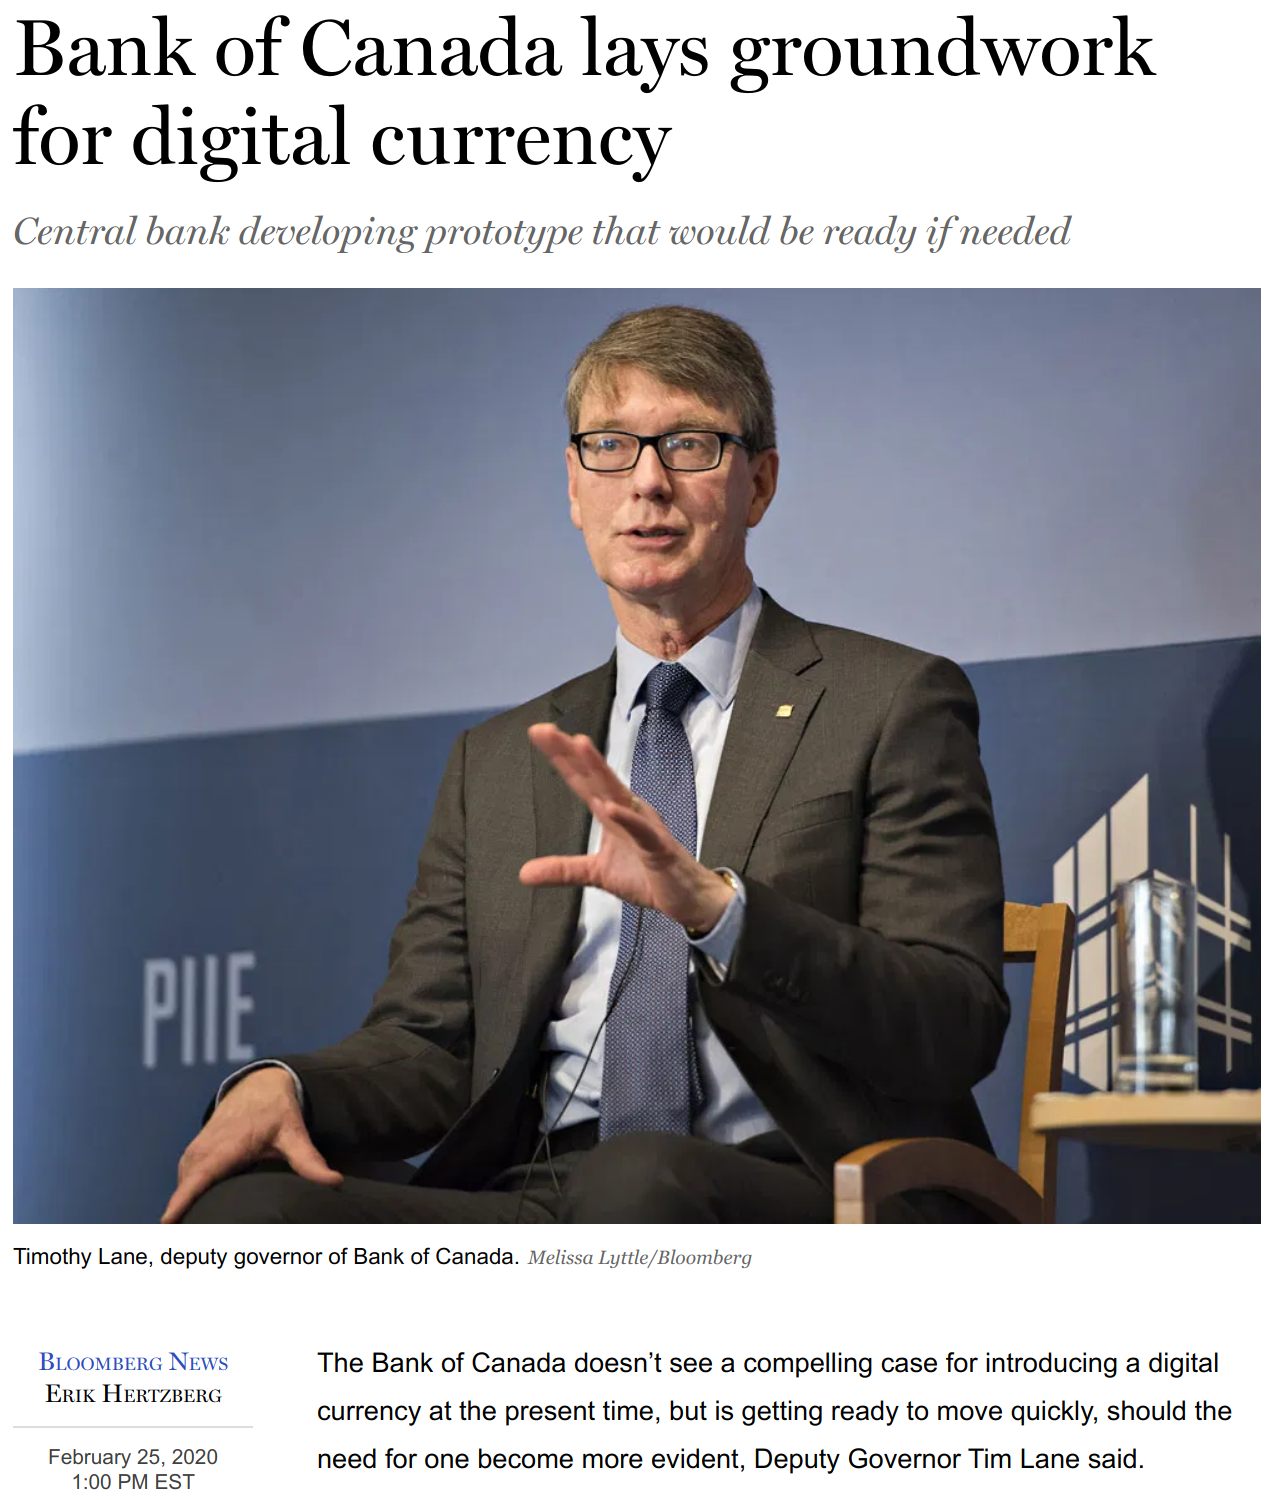
\includegraphics[height=6.5cm]{../pics/cryptocurrency/fp2020-02-boc}
        \caption{\cite{financialpost2020:bankofcandacrypto}}
	\end{figure}
}

\frame{
  \frametitle{Six central banks to collaborate on digital currency research}
	\begin{figure}
        \centering
		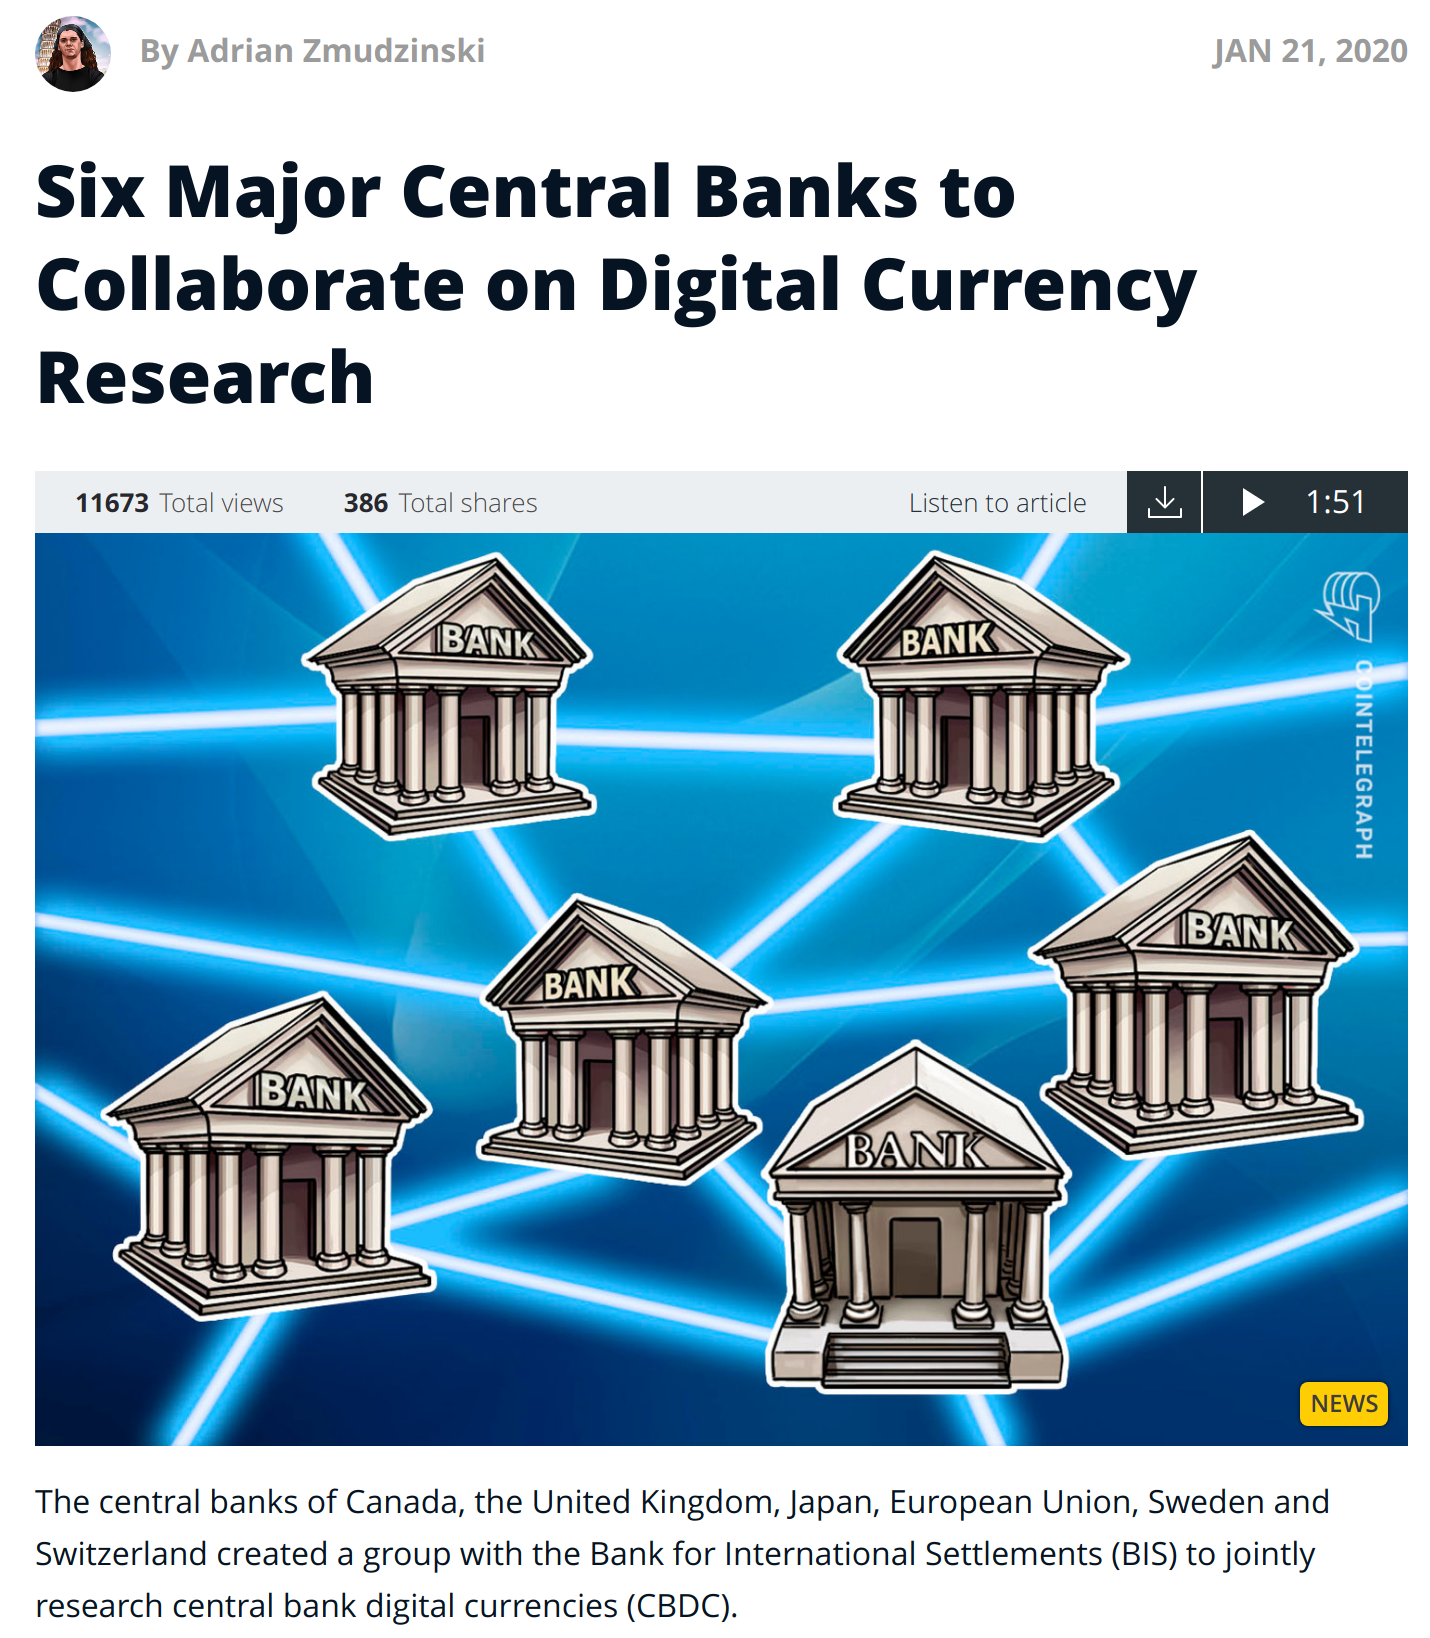
\includegraphics[height=5.5cm]{../pics/cryptocurrency/cointelegraph-2020-01-bis}
        \caption{\cite{cointelegraph:bis}}
	\end{figure}
  ``The central banks of Canada, the United Kingdom, Japan, European Union, Sweden and Switzerland created a group with the Bank for International Settlements (BIS) to jointly research central bank digital currencies (CBDC).''
}

\frame{
	\frametitle{The People's Bank of China}
	\begin{figure}
        \centering
		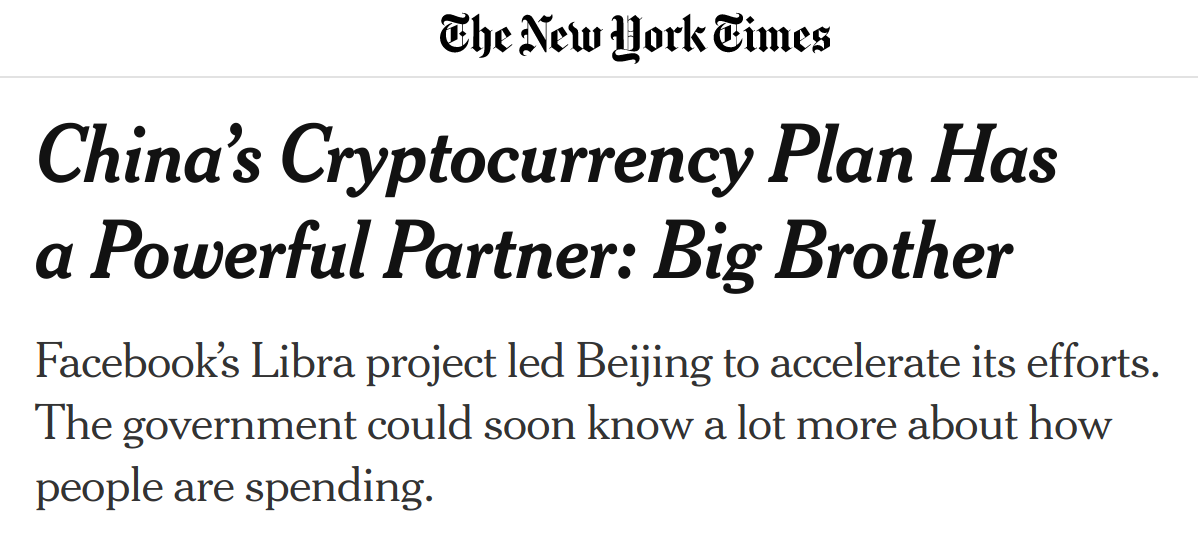
\includegraphics[width=11.5cm]{../pics/cryptocurrency/nytimes2019-china-crypto}
        \caption{\cite{nytimes2019:china-crypto}}
%        \caption{\url{https://www.nytimes.com/2019/10/18/technology/china-cryptocurrency-facebook-libra.html}}
	\end{figure}
    See also \citeauthor{forbes201908:chinacrypto}'s article in Forbes (\citeyear{forbes201908:chinacrypto}).
% also check   https://www.forbes.com/sites/michaeldelcastillo/2019/08/27/alibaba-tencent-five-others-to-recieve-first-chinese-government-cryptocurrency/#1fb606111a51
% "In addition to preventing regional banks and other organizations from being disintermediated, Mu said the two-tiered system is designed to “curb” public demand for other cryptographic assets, consolidate China’s national currency sovereignty, ensure that the central bank maintains control over monetary policy affecting the currency, increase the likelihood of people using the currency, distribute the risk of having all the authority directly in the hands of the central bank and encourage competition between the organizations that receive the cryptocurrency."
}

\frame{
    \frametitle{Other countries}
    \begin{itemize}
        \item Switzerland
        \item Sweden
        \item Singapore
        \item Philipines
    \end{itemize}
}



